

\section{Roteador TP-Link Wireless N150}
\label{roteador_01}


\begin{table}[ht!]

	\begin{tabular}{r l|l p{12cm} }
		
		\textcolor{gray}{Especificação} &&& 	{Roteador TP-Link Wireless N150}\\
		\textcolor{gray}{Data} &&& 				{31/10/2014}\\
        \textcolor{gray}{Beneficiado} &&&		{Universidata Informatica e
        Telefonia LTDA}
        \\
        \textcolor{gray}{CNPJ} &&& 				{39.121.694/0001-50} \\
        \textcolor{gray}{Número Nota} &&& 		{00.722.402} \\
		\textcolor{gray}{Quantidade} &&& 		{-} \\
		\textcolor{gray}{Valor} &&& 			{R\$95,00} \\
		\textcolor{gray}{Data Sheet} &&& 		{-} \\

		\textcolor{gray}{Função no projeto} &&& {O roteador wireless será responsável
		por estabelecer a comunicação ethernet entre o computador da base (ROCK) e o
		tablet (Android) utilizado pelo operador,}
		\\
		\textcolor{gray}{Razão da Escolha} &&& {Proximidade com o LEAD e pronta
		entrega.}

	\end{tabular}
\end{table}

\newpage
\subsection{Foto do Material}
\begin{figure}[H]
 \centering
 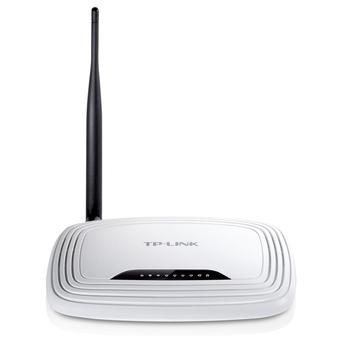
\includegraphics[width=1\columnwidth]{Roteador/foto.jpg}
 \caption{Roteador TP-Link Wireless N150}
\end{figure}

\subsection{Nota Fiscal}
\begin{figure}[H]
 \centering
 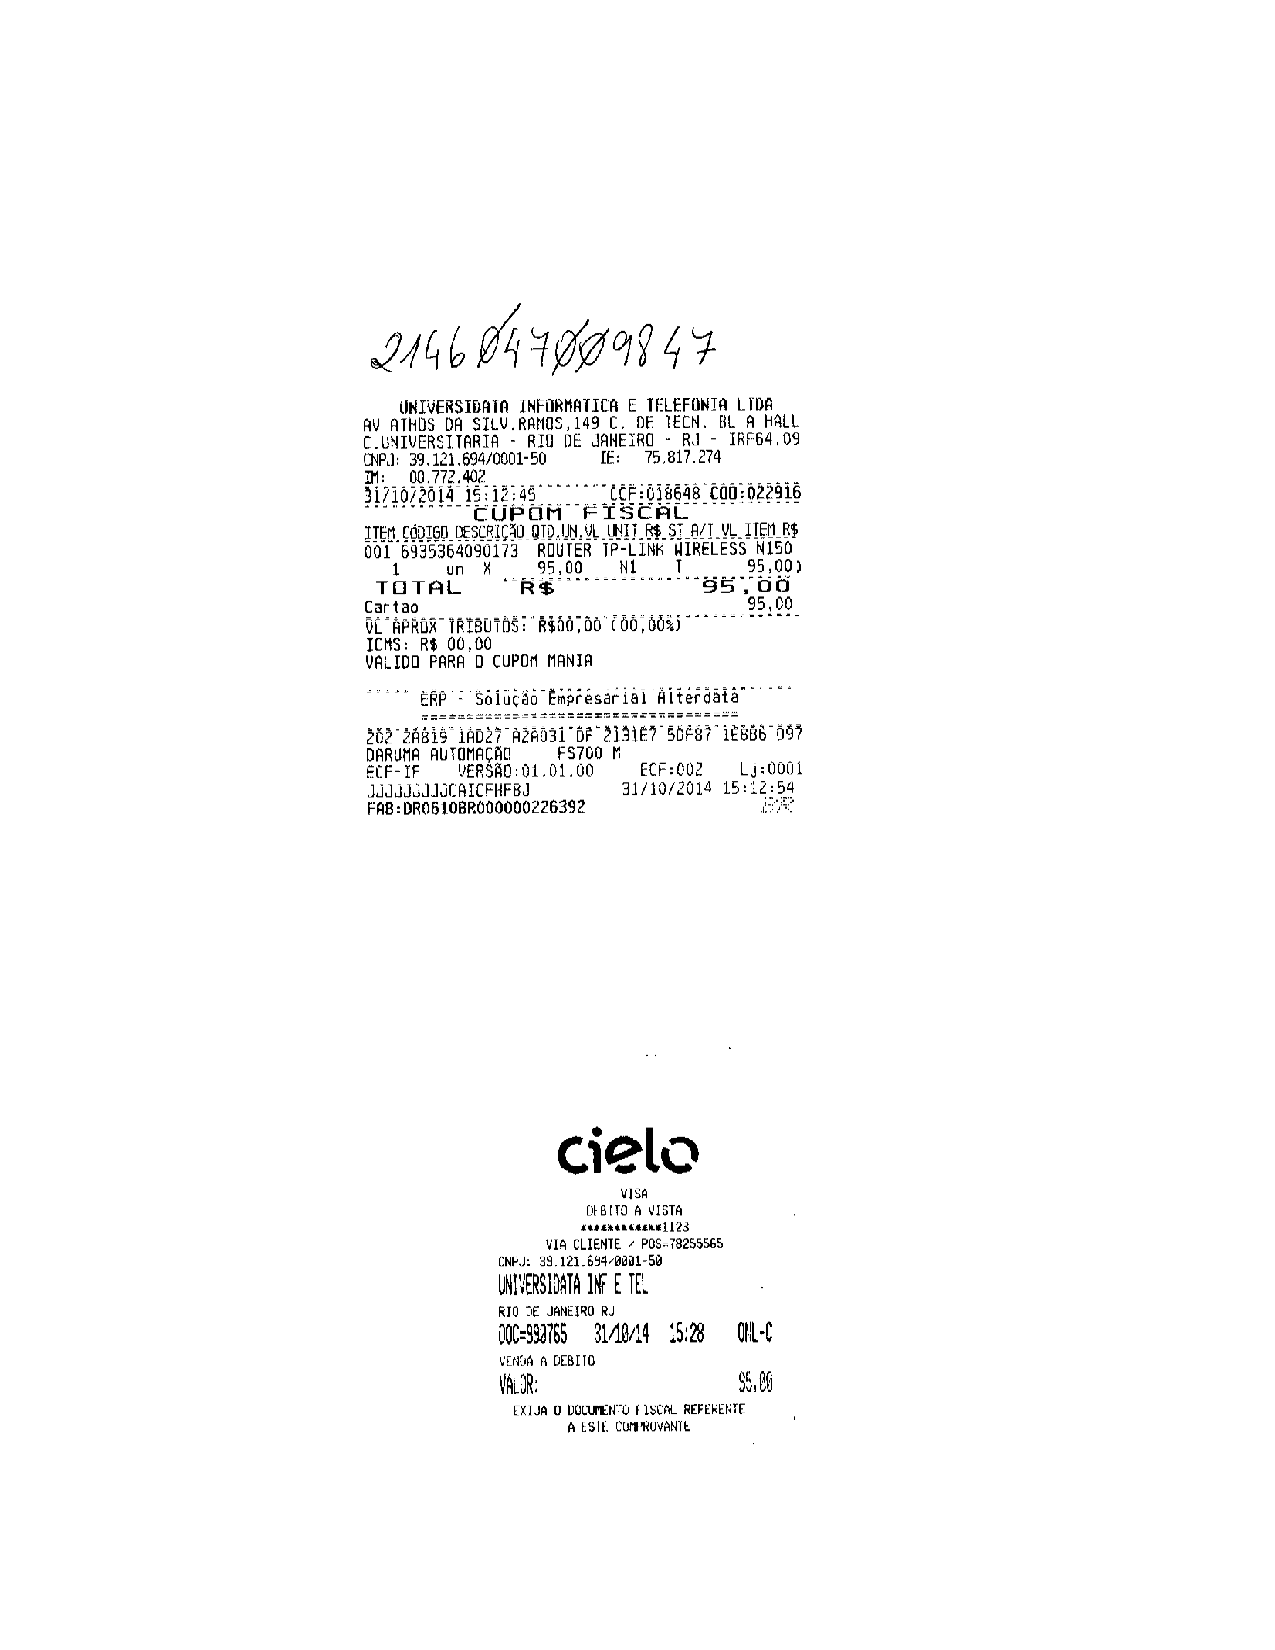
\includegraphics[width=0.9\columnwidth]{Roteador/nota_universidata.pdf}
 \caption{Nota fiscal do Roteador TP-Link Wireless N150}
 \end{figure}